\documentclass[12pt]{article}

\usepackage{graphicx}
\usepackage{geometry}
\usepackage{float}
\usepackage[italian]{babel}
\usepackage[linktoc=all,hidelinks]{hyperref}
\usepackage{xcolor}
\usepackage{upquote}


\geometry{a4paper, top = 3 cm, bottom = 3 cm, left = 2.5 cm, right = 2.5 cm}
\setlength{\parindent}{0pt}


\title{Guida per la creazione di istanze su AWS}

\author{Originale di Stefano Raimondo Usai, Revisione di Costantino}

\date{\today}


\begin{document}

\maketitle

\newpage

\tableofcontents

\newpage

\section{Introduzione}

Questa guida prende spunto dal "Report del progetto per Big Data di Senis Martina e Tola Alessandro" per creare due istanze sul servizio EC2 di Amazon AWS e installarci Apache Hadoop e Apache Spark.

Questa è una versione aggiornata della guida originale scritta da Stefano Raimondo Usai il 5 Ottobre 2019.

Per proporre miglioramenti o correzioni, il codice sorgente di questa guida è disponibile \underline{\href{https://github.com/costantino2000/big-data-aws-guide}{su GitHub}}.


\newpage

\section{Creazione delle istanze AWS}

Creiamo il nostro account AWS al \underline{\href{https://aws.amazon.com/it/}{seguente link}} e accediamo per raggiungere la console di AWS:

\begin{figure}[H]
    \centering
    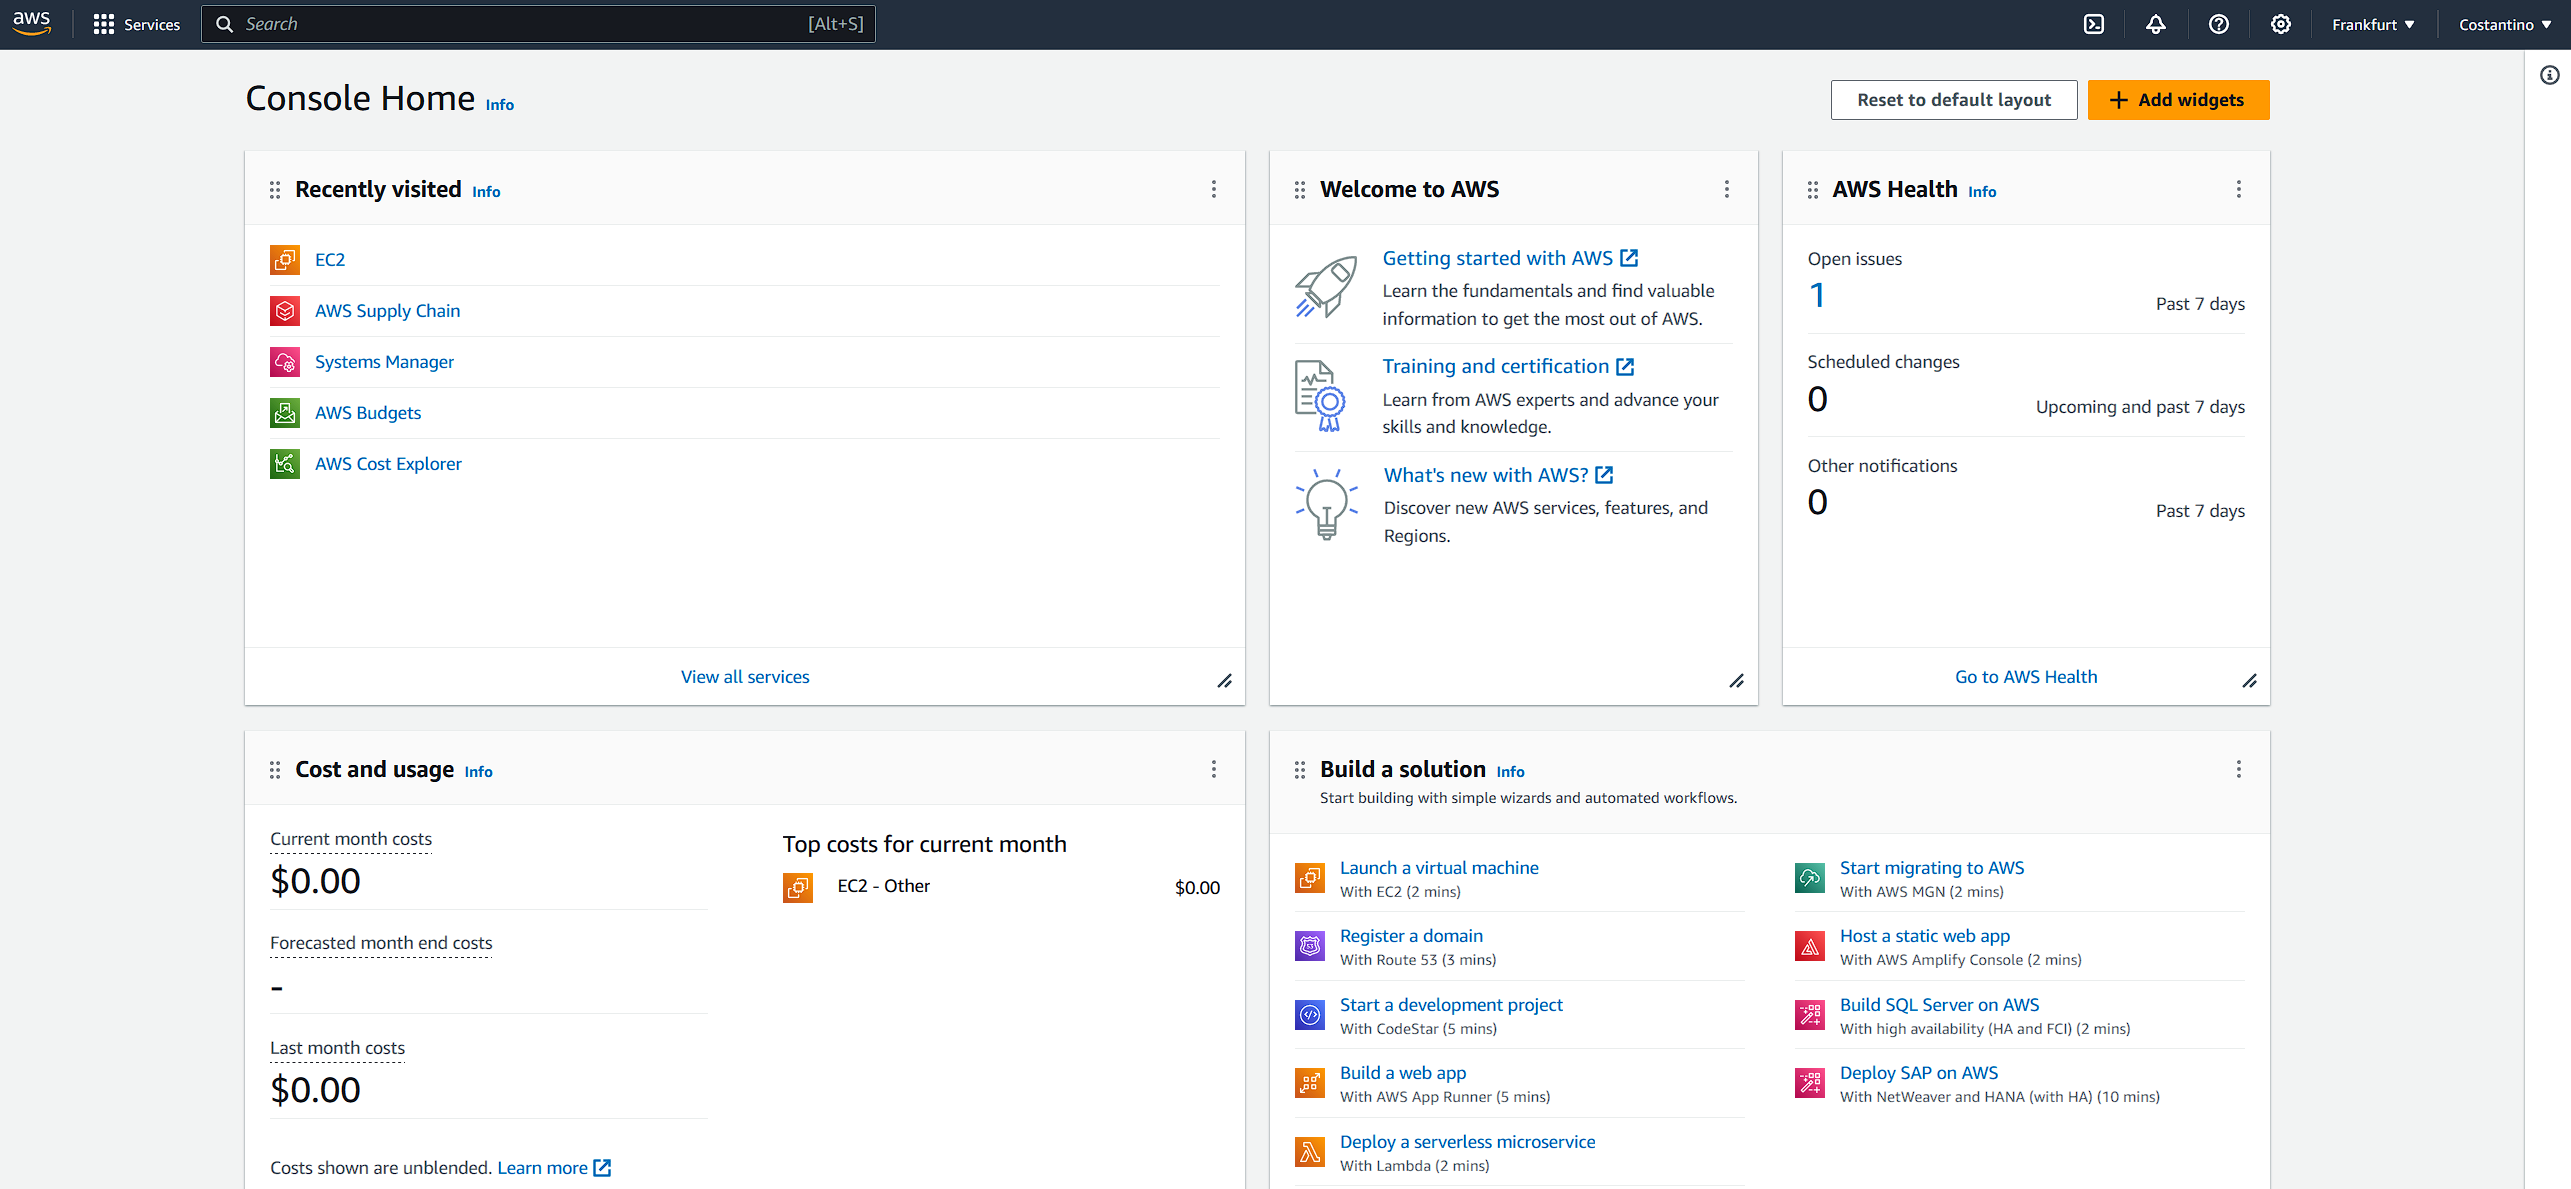
\includegraphics[width=0.95\textwidth]{images/aws-console.png}
\end{figure}

Amazon fornisce una serie di servizi. Quello che andremo a utilizzare noi è \textbf{Amazon Elastic Compute Cloud} (\textbf{Amazon EC2}), il quale offre un piano gratuito che include 750 ore mensili per l'utilizzo di istanze t2.micro Linux e Windows per un anno.

Una volta nella \textbf{dashboard di EC2} (che si può raggiungere tramite la barra di ricerca della console), selezioniamo il pulsante arancione \textbf{Launch instance}, e iniziamo così la creazione delle istanze.
Nella sezione \textbf{Application and OS Images} ci viene permesso di scegliere il tipo di sistema che vogliamo per le nostre istanze (le istanze che rientrano nel piano delle 750 ore sono quelle che riportano la scritta \textit{Free tier eligible}). Per una questione di semplicità la scelta del sistema operativo è ricaduta su \textbf{Ubuntu 22.04}:

\begin{figure}[H]
    \centering
    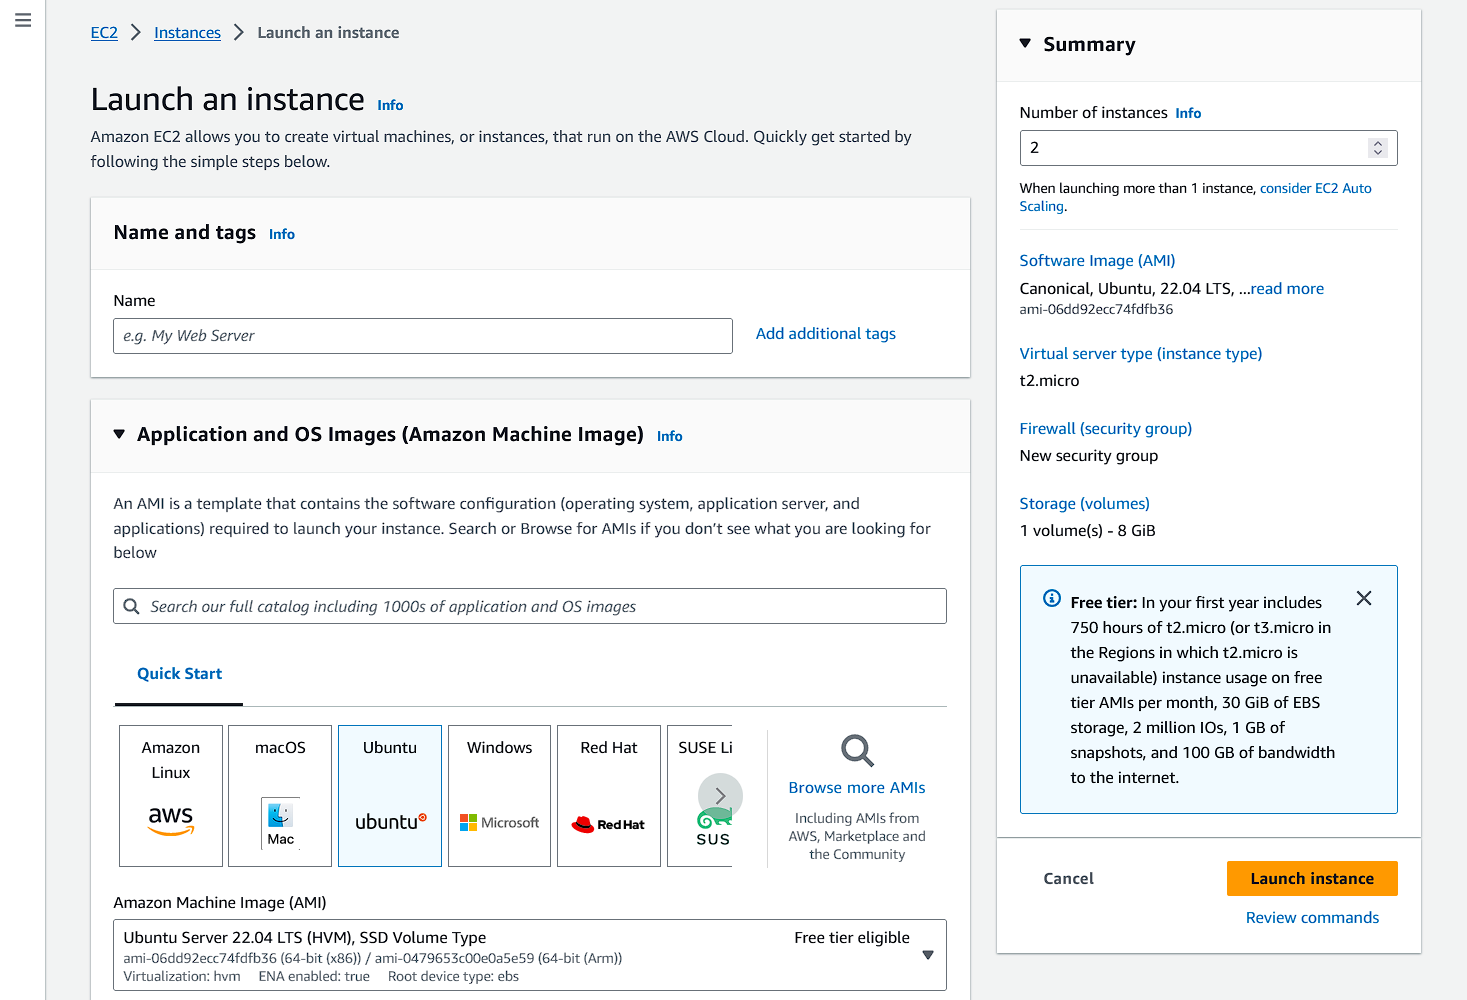
\includegraphics[width=0.8\textwidth]{images/vm-selection.png}
\end{figure}

Scelto il sistema operativo proseguiamo fino alla sezione \textbf{Instance type} e assicuriamoci che l'opzione selezionata sia \textbf{t2.micro} (l'unica \textit{Free tier eligible}):

\begin{figure}[H]
    \centering
    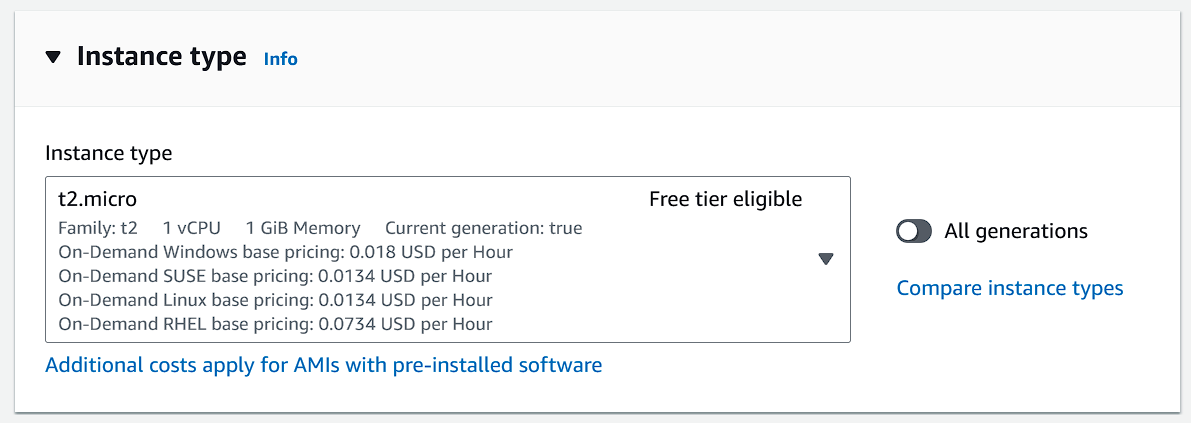
\includegraphics[width=0.65\textwidth]{images/instance-type.png}
\end{figure}

Proseguiamo da qui nella configurazione delle istanze raggiungendo la sezione \textbf{Key pair (login)} e clicchiamo su \textbf{Create a new key pair}:

\begin{figure}[H]
    \centering
    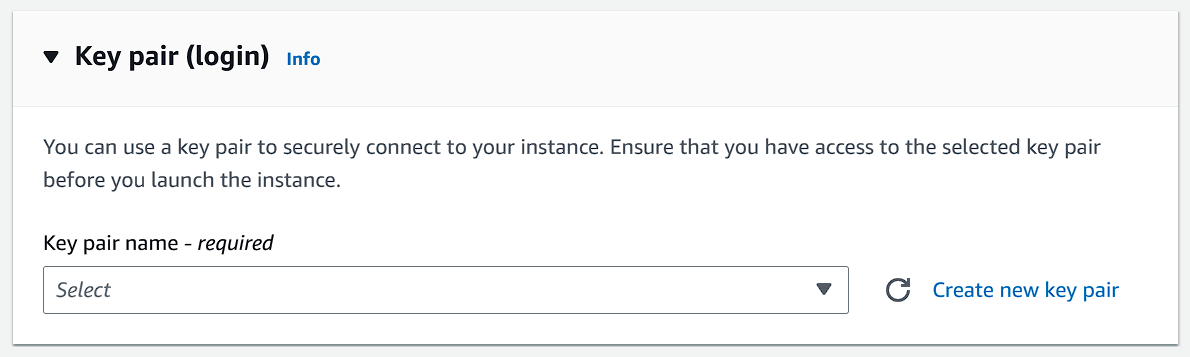
\includegraphics[width=0.65\textwidth]{images/key-pair.png}
\end{figure}

Nel popup che si aprirà impostiamo come nome \textbf{my-key}, come tipo di chiave \textbf{RSA} e come formato \textbf{.pem}:

\begin{figure}[H]
    \centering
    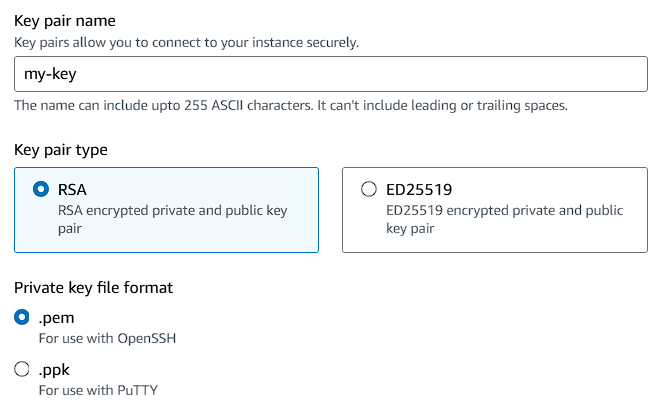
\includegraphics[width=0.65\textwidth]{images/key-creation.png}
\end{figure}

Vi verrà chiesto di salvare questa chiave sul computer. È molto importante salvarla in un posto sicuro, perché senza non è possibile accedere alle istanze da terminale (vi è la possibilità di farlo dal sito ma non è molto comodo).

Nota: se vi trovate su una distribuzione Linux o Mac dovrete settare il permesso alla chiave con il comando seguente:

\begin{verbatim}
    $ chmod 400 my-key.pem
\end{verbatim}

Raggiungiamo ora la sezione \textbf{Network settings} e clicchiamo sul pulsante \textbf{Edit} in alto a destra:

\begin{figure}[H]
    \centering
    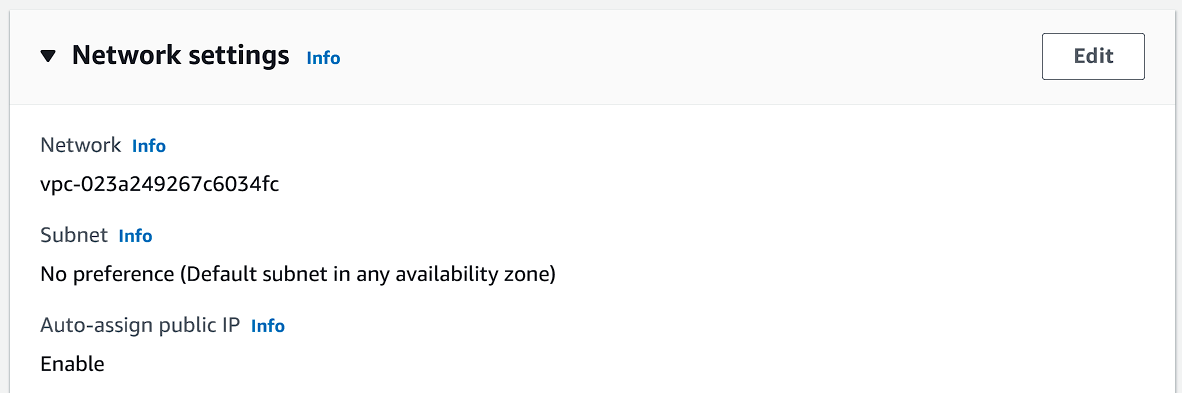
\includegraphics[width=0.65\textwidth]{images/network.png}
\end{figure}

Tramite il pulsante che apparirà in fondo alla sezione (\textbf{Add security group rule}) creiamo una seconda regola per le porte da utilizzare nelle nostre istanze. Scegliamo per il tipo l'opzione \textbf{All traffic} e per il tipo di sorgente la voce \textbf{Anywhere}. Alla fine dovremmo avere una seconda regola come appare nella seguente figura:

\begin{figure}[H]
    \centering
    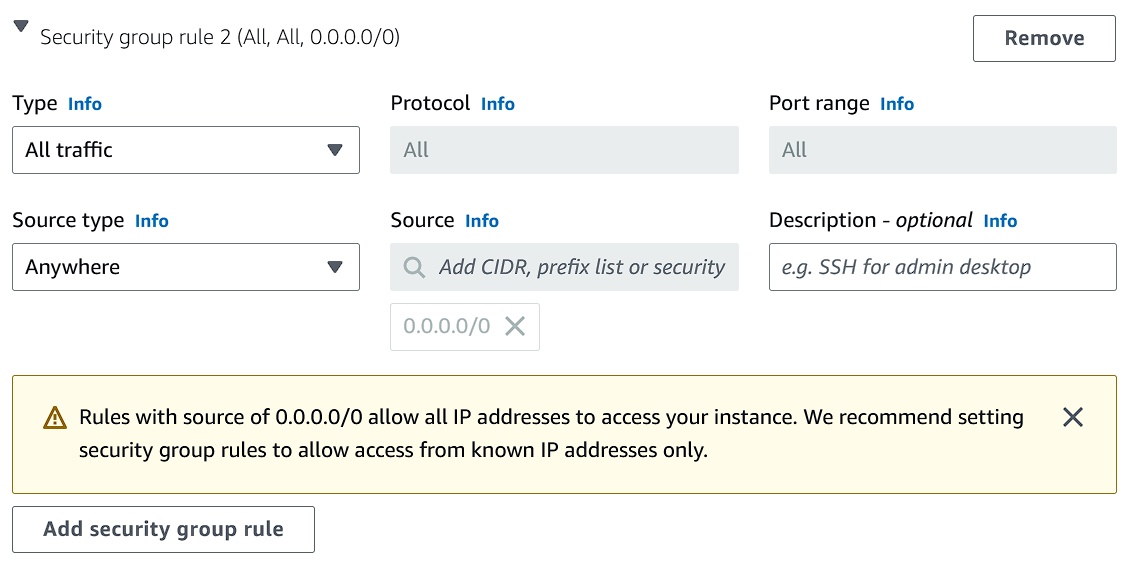
\includegraphics[width=0.65\textwidth]{images/security-rule.png}
\end{figure}

Dal sommario (in alto a destra o in fondo alla pagina, a seconda della dimensione della finestra del browser) impostiamo infine il numero di istanze a \textbf{2}, e clicchiamo sul pulsante \textbf{Launch instance} per crearle.

Verremo riportati alla schermata con l'elenco delle istanze, dove potremmo rinominare le due nuove istanze appena create. Chiamiamo l'istanza master \textbf{namenode} e quella slave \textbf{datanode2}. Fatto questo selezioniamo le istanze e avviamole dal menu a tendina del pulsante \textbf{Instance state} (se non si stanno già avviando):

\begin{figure}[H]
    \centering
    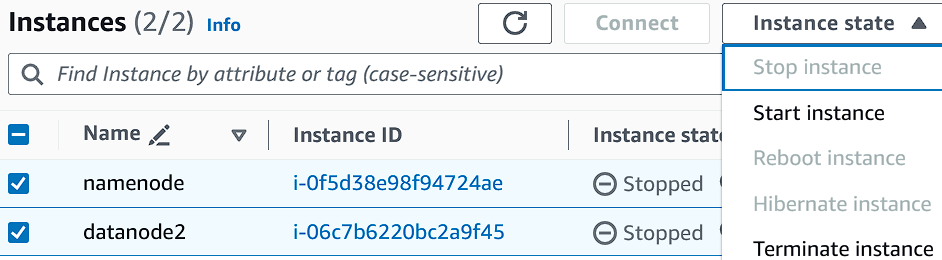
\includegraphics[width=0.7\textwidth]{images/activate-instance.png}
\end{figure}

Selezionando un'istanza alla volta e cliccando sul tasto \textbf{Connect} apparirà una schermata per la connessione. Andando nella sezione \textbf{SSH client} si può trovare il comando ssh con cui connettersi alla istanza selezionata che è possibile copiare per comodità:

\begin{figure}[H]
    \centering
    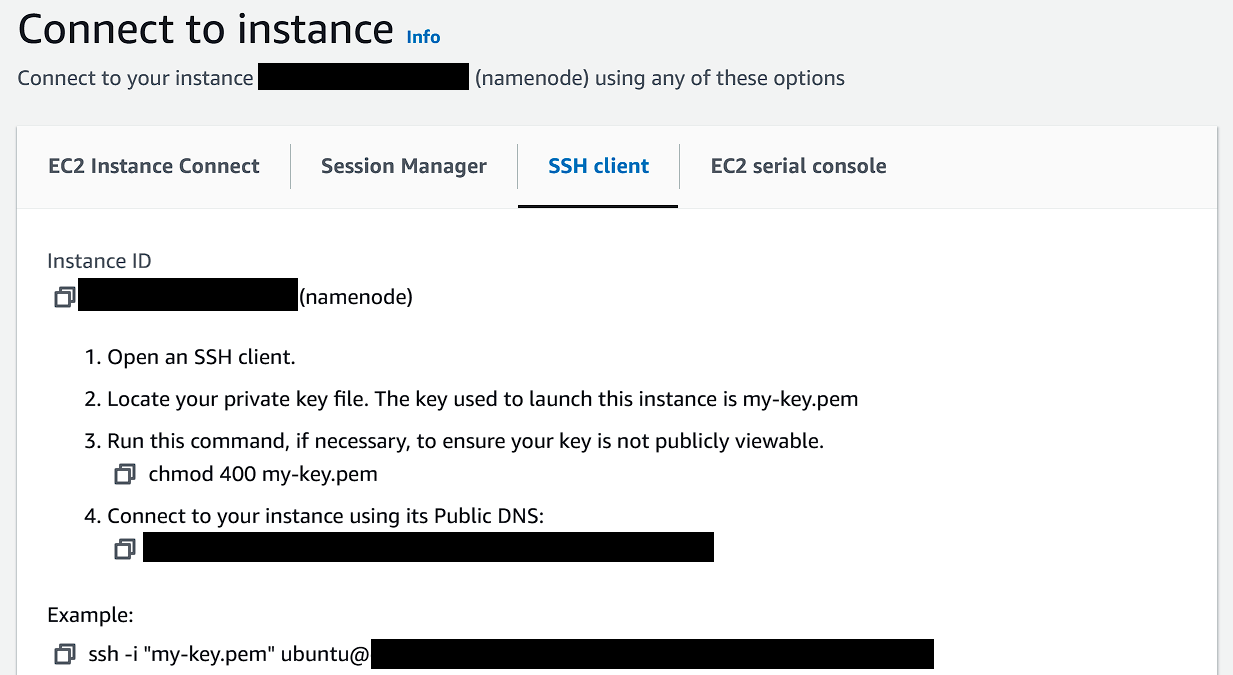
\includegraphics[width=0.7\textwidth]{images/instance-connect.png}
\end{figure}

Aprendo un terminale sul nostro computer potremo incollare il comando mostrato oppure digitarlo manualmente nel seguente modo (assicurandoci di essere nella cartella dove risiede il file della chiave, e con ADDRESS indichiamo l'indirizzo pubblico IPv4 che si può trovare nei dettagli dell'istanza selezionata):

\begin{verbatim}
    $ ssh -i my-key.pem ubuntu@ADDRESS
\end{verbatim}

Infine, per trasferire la chiave RSA nell'istanza master senza l'utilizzo di S3, possiamo utilizzare il seguente comando (con un secondo terminale e sempre dalla cartella in cui è presente la chiave):

\begin{verbatim}
    $ scp -i my-key.pem my-key.pem ubuntu@ADDRESS:/home/ubuntu/.ssh
\end{verbatim}

In questa maniera, in caso si dovesse perdere la chiave, si potrà accedere all'istanza dalla sezione \textbf{Ec2 Instance Connect} dello screenshot precedente (che permette di connettersi con un terminale web), e andando nella cartella \textbf{/home/ubuntu/.ssh} si ritroverà il file della chiave, che si potrà aprire con nano per recuperarne il contenuto e ri-salvarlo sul proprio computer come file .pem.


\newpage

\section{Configurazione dei cluster}


\subsection{Download di Hadoop e installazione di Java}

Torniamo nelle console collegate tramite SSH alle nostre due istanze. \textcolor{red}{In ognuna delle istanze} bisogna aggiornare per prima cosa i repository (potrebbe chiedere di riavviare dei servizi in caso di aggiornamento del kernel, basta accettare le impostazioni di default e fare ok):

\begin{verbatim}
    $ sudo apt-get update && sudo apt-get dist-upgrade -y
\end{verbatim}

e installare Java 8:

\begin{verbatim}
    $ sudo apt-get install openjdk-8-jdk -y
\end{verbatim}

Scarichiamo ora il file compresso di Hadoop, estraiamolo e spostiamolo nella cartella \textbf{/home/ubuntu/hadoop}. Infine, rimuoviamo il file scaricato in precedenza (occhio ai \textbf{comandi su più righe}, vanno riportati su una prima di eseguirli!):

\begin{verbatim}
    $ wget https://archive.apache.org/dist/hadoop/common/hadoop-2.7.7
        /hadoop-2.7.7.tar.gz
    $ sudo tar zxvf hadoop-2.7.7.tar.gz
    $ sudo mv ./hadoop-2.7.7 /home/ubuntu/hadoop
    $ rm hadoop-2.7.7.tar.gz
\end{verbatim}

Impostiamo le variabili di ambiente aprendo il file \textbf{.profile}:

\begin{verbatim}
    $ nano /home/ubuntu/.profile
\end{verbatim}

e inserendoci le seguenti righe:

\begin{verbatim}
    export JAVA_HOME=/usr/lib/jvm/java-8-openjdk-amd64
    export PATH=$PATH:$JAVA_HOME/bin
    export HADOOP_HOME=/home/ubuntu/hadoop
    export PATH=$PATH:/home/ubuntu/hadoop/bin
    export HADOOP_CONF_DIF=/home/ubuntu/hadoop/etc/hadoop
    export PYSPARK_PYTHON=python3
\end{verbatim}

Infine aggiorniamole utilizzando il comando \textbf{source}:

\begin{verbatim}
    $ source /home/ubuntu/.profile
\end{verbatim}


\newpage


\subsection{Configurazione della connessione SSH}

Questa parte andrà svolta \textcolor{red}{solo sull'istanza del master}. Creiamo un file di configurazione per associare i nomi delle istanze ai loro indirizzi IPv4 pubblici e alla loro chiave privata:

\begin{verbatim}
    $ nano /home/ubuntu/.ssh/config
\end{verbatim}

Identifichiamo con \textbf{namenode} il master e con \textbf{datanode1} e \textbf{datanode2} i due slave. I primi due gireranno sull'istanza namenode, mentre datanode2 girerà sull'istanza omonima:

\begin{verbatim}
    Host namenode
    HostName namenode
    User ubuntu
    IdentityFile /home/ubuntu/.ssh/my-key.pem
    Host datanode1
    HostName namenode
    User ubuntu
    IdentityFile /home/ubuntu/.ssh/my-key.pem
    Host datanode2
    HostName datanode2
    User ubuntu
    IdentityFile /home/ubuntu/.ssh/my-key.pem
\end{verbatim}

Ora apriamo \textcolor{red}{in entrambe le istanze} il file \textbf{hosts}:

\begin{verbatim}
    $ sudo nano /etc/hosts
\end{verbatim}

e andiamo a includere gli ip pubblici in questo modo:

\begin{verbatim}
    IPMASTER namenode
    IPMASTER datanode1
    IPSLAVE  datanode2
\end{verbatim}

Dove IPMASTER e IPSLAVE si trovano selezionando singolarmente ognuna delle istanze nella dashboard di EC2 e leggendo dal pannello dei dettagli la voce IPv4 Public IP (come già visto nella sezione 2). Facendo cosi, quando fermeremo le istanze e le rifaremo partire, dato che avranno indirizzi ip pubblici diversi, basterà aggiornare il file hosts in entrambe le istanze con i nuovi indirizzi ip pubblici.

Ritorniamo ora \textcolor{red}{al terminale del master}, e diamo le autorizzazioni SSH per la connessione dal master allo slave:

\begin{verbatim}
    $ ssh-keygen -f /home/ubuntu/.ssh/id_rsa -t rsa -P ''
    $ cat /home/ubuntu/.ssh/id_rsa.pub
        >> /home/ubuntu/.ssh/authorized_keys
    $ chmod 600 /home/ubuntu/.ssh/my-key.pem
    $ ssh datanode1 'cat >> /home/ubuntu/.ssh/authorized_keys'
        < /home/ubuntu/.ssh/id_rsa.pub
    $ ssh datanode2 'cat >> /home/ubuntu/.ssh/authorized_keys'
        < /home/ubuntu/.ssh/id_rsa.pub
\end{verbatim}

Per verificare che tutti i passaggi siano stati eseguiti correttamente e che la connessione SSH sia attiva possiamo provare il seguente comando (sempre dal terminale del master):

\begin{verbatim}
    $ ssh datanode2
\end{verbatim}

Questo verifica che la connessione verso l'istanza slave funzioni correttamente (in caso negativo il terminale restituirà il messaggio \textbf{PERMISSION DENIED}). Per controllare datanode1 basta cambiare il numero.

Una volta avviata una connessione la si può interrompere in qualsiasi momento con la combinazione \textcolor{red}{ctrl+D}.


\subsection{Configurazione di Hadoop e Spark}



\subsubsection{Configurazione di tutti i nodi}

\textcolor{red}{Per ogni istanza} si devono modificare quattro file di configurazione. Il primo, \textbf{hadoop-env.sh}, contiene la configurazione delle variabili di ambiente di Hadoop. Apriamolo:

\begin{verbatim}
    $ nano $HADOOP_CONF_DIF/hadoop-env.sh
\end{verbatim}

e sostituiamo la riga

\begin{verbatim}
    export JAVA_HOME=$JAVA_HOME
\end{verbatim}

con

\begin{verbatim}
    export JAVA_HOME=/usr/lib/jvm/java-8-openjdk-amd64
\end{verbatim}

Passiamo al secondo file, \textbf{core-site.xml}. Apriamolo:

\begin{verbatim}
    $ sudo nano $HADOOP_CONF_DIF/core-site.xml
\end{verbatim}

e inseriamo la seguente proprietà all'interno dell'elemento \textbf{\textlangle configuration\textrangle}, con al posto di HOSTNAME l'indirizzo Ipv4 \textbf{privato} del master (reperibile nella stessa schermata da cui si è preso quello pubblico):

\begin{verbatim}
    <property>
    <name>fs.defaultFS</name>
    <value>hdfs://HOSTNAME:9000</value>
    </property>
\end{verbatim}

Il terzo file, \textbf{yarn-site.xml}, serve a impostare su quale macchina girerà il source manager. Apriamolo:

\begin{verbatim}
    $ sudo nano $HADOOP_CONF_DIF/yarn-site.xml
\end{verbatim}

e, come fatto prima, inseriamo la seguente proprietà:

\begin{verbatim}
    <property>
    <name>yarn.nodemanager.aux-services</name>
    <value>mapreduce_shuffle</value>
    </property>
    <property>
    <name>yarn.resourcemanager.hostname</name>
    <value>namenode</value>
    </property>
\end{verbatim}

Infine, creiamo una copia del file \textbf{mapred-site.xml.template} e apriamolo:

\begin{verbatim}
    $ sudo cp $HADOOP_CONF_DIF/mapred-site.xml.template
        $HADOOP_CONF_DIF/mapred-site.xml
    $ sudo nano $HADOOP_CONF_DIF/mapred-site.xml
\end{verbatim}

per inserire la seguente proprietà:

\begin{verbatim}
    <property>
    <name>mapreduce.jobtracker.address</name>
    <value>namenode:54311</value>
    </property>
    <property>
    <name>mapreduce.framework.name</name>
    <value>yarn</value>
    </property>
\end{verbatim}



\subsubsection{Configurazione dell'istanza master}

Andiamo \textcolor{red}{nel terminale del master} e apriamo il file \textbf{hdfs-site.xml}:

\begin{verbatim}
    $ sudo nano $HADOOP_CONF_DIF/hdfs-site.xml
\end{verbatim}

per inserire la seguente proprietà (dentro il tag \textit{configuration} come fatto finora):

\begin{verbatim}
    <property>
    <name>dfs.replication</name>
    <value>2</value>
    </property>
    <property>
    <name>dfs.namenode.name.dir</name>
    <value>file:///home/ubuntu/hadoop/data/hdfs/namenode</value>
    </property>
    <property>
    <name>dfs.datanode.data.dir</name>
    <value>file:///home/ubuntu/hadoop/data/hdfs/datanode</value>
    </property>
\end{verbatim}

Creiamo ora le cartelle in cui andranno contenuti i dati del master e del nodo attivo sull'istanza master (datanode1):

\begin{verbatim}
    $ sudo mkdir -p $HADOOP_HOME/data/hdfs/namenode
    $ sudo mkdir -p $HADOOP_HOME/data/hdfs/datanode
    $ sudo nano $HADOOP_CONF_DIF/masters
\end{verbatim}

e scriviamoci dentro il nome del master:

\begin{verbatim}
    namenode
\end{verbatim}

Apriamo poi il file degli slave:

\begin{verbatim}
    $ sudo nano $HADOOP_CONF_DIF/slaves
\end{verbatim}

e scriviamoci i nomi degli slave (se contiene \textit{localhost} lo si può rimuovere senza problemi):

\begin{verbatim}
    datanode1
    datanode2
\end{verbatim}

Infine diamo all'utente \textit{ubuntu} la proprietà della cartella in cui si trova la home di Hadoop:

\begin{verbatim}
    $ sudo chown -R ubuntu $HADOOP_HOME
\end{verbatim}



\subsubsection{Configurazione dell'istanza datanode2}

Andiamo nel terminale \textcolor{red}{della seconda istanza} e apriamo il file \textbf{hdfs-site.xml}:

\begin{verbatim}
    $ sudo nano $HADOOP_CONF_DIF/hdfs-site.xml
\end{verbatim}

per inserire la seguente proprietà nella configurazione:

\begin{verbatim}
    <property>
    <name>dfs.replication</name>
    <value>2</value>
    </property>
    <property>
    <name>dfs.namenode.name.dir</name>
    <value>file:///home/ubuntu/hadoop/data/hdfs/namenode</value>
    </property>
    <property>
    <name>dfs.datanode.data.dir</name>
    <value>file:///home/ubuntu/hadoop/data/hdfs/datanode</value>
    </property>
\end{verbatim}

Creiamo poi nel nodo la cartella in cui andranno contenuti i dati dello slave:

\begin{verbatim}
    $ sudo mkdir -p $HADOOP_HOME/data/hdfs/datanode
\end{verbatim}

e diamo all'utente \textit{ubuntu} la proprietà della cartella in cui si trova la home di Hadoop:

\begin{verbatim}
    $ sudo chown -R ubuntu $HADOOP_HOME
\end{verbatim}




\subsubsection{Installazione e configurazione di Spark}

L'installazione di Spark va fatta \textcolor{red}{su ogni nodo del cluster}. Scarichiamo ed estraiamo
Spark spostandolo nella cartella \textbf{/home/ubuntu/spark}, e alla fine rimuoviamo il
file .tgz scaricato:

\begin{verbatim}
    $ wget https://archive.apache.org/dist/spark
        /spark-3.2.4/spark-3.2.4-bin-hadoop2.7.tgz
    $ tar xvzf spark-3.2.4-bin-hadoop2.7.tgz
    $ sudo mv ./spark-3.2.4-bin-hadoop2.7 /home/ubuntu/spark
    $ rm spark-3.2.4-bin-hadoop2.7.tgz
\end{verbatim}

Per impostare le variabili d'ambiente di Spark (che includono la configurazione di Hadoop) cloniamo e apriamo il file \textbf{spark-env.sh}:

\begin{verbatim}
    $ sudo cp spark/conf/spark-env.sh.template spark/conf/spark-env.sh
    $ sudo nano spark/conf/spark-env.sh
\end{verbatim}

e inseriamo le seguenti righe, sostituendo NAMENODEADDRESS con l'indirizzo privato del master:

\begin{verbatim}
    export SPARK_MASTER_HOST="NAMENODEADDRESS"
    export HADOOP_CONF_DIR="/home/ubuntu/hadoop/conf"
\end{verbatim}



\newpage

\section{Esecuzione dei programmi}



\subsection{Primo avvio di Hadoop}

Questi comandi andranno lanciati \textcolor{red}{solo sul master}. Per prima cosa formattiamo la partizione dell'hdfs:

\begin{verbatim}
    $ hdfs namenode -format
\end{verbatim}

Poi bisogna avviare i servizi \textbf{hdfs}, \textbf{yarn} e \textbf{historyserver} con i seguenti comandi (in alternativa c'è lo script deprecato \textbf{start-all.sh}):

\begin{verbatim}
    $ $HADOOP_HOME/sbin/start-dfs.sh
    $ $HADOOP_HOME/sbin/start-yarn.sh
    $ $HADOOP_HOME/sbin/mr-jobhistory-daemon.sh start historyserver
\end{verbatim}

Per essere sicuri infine che hdfs sia configurato e funzioni correttamente si esegue comando seguente:

\begin{verbatim}
    $ hdfs dfsadmin -report
\end{verbatim}

Se tutto ha funzionato correttamente dovrebbero esserci \textbf{due datanode live}. Se questo avviene, dentro la cartella \textbf{\$HADOOP\_HOME/hdfs} dovrebbe essere presente la cartella \textbf{data}, la quale dovrebbe contenere le cartelle \textbf{datanode} e/o \textbf{namenode} (nel nodo master ci sono entrambe, nello slave solo la seconda), le quali a loro volta dovrebbero contenere il file \textbf{in\_use.lock} e la cartella \textbf{current}.



\subsection{Primo avvio di Spark}

Prima di avviare Spark è necessario fermare i processi di Hadoop (sempre \textcolor{red}{dal terminale del master}), in quanto le istanze gratuite di AWS non hanno abbastanza ram per eseguirli entrambi in contemporanea (in alternativa ai comandi seguenti c'è lo script deprecato \textbf{stop-all.sh}):

\begin{verbatim}
    $ $HADOOP_HOME/sbin/stop-dfs.sh
    $ $HADOOP_HOME/sbin/stop-yarn.sh
    $ $HADOOP_HOME/sbin/mr-jobhistory-daemon.sh stop historyserver
\end{verbatim}

Avviamo ora Spark con il seguente comando:

\begin{verbatim}
    $ /home/ubuntu/spark/sbin/start-master.sh
\end{verbatim}

A questo punto dobbiamo aprire l'interfaccia web di Spark. Apriamo il nostro browser, andiamo all'indirizzo pubblico del master seguito dalla porta 8080 (quindi \textbf{ip\_pubblico:8080}) e salviamo l'URL indicato nel titolo della pagina (quello che inizia con \textbf{spark://...}). Useremo questo indirizzo per lanciare gli slave.

Nel terminale \textcolor{red}{di ogni nodo slave} (quindi anche nell'istanza del master, dato che contiene datanode1) deve essere inserito il comando seguente, sostituendo ADDRESS con l'URL trovato prima:

\begin{verbatim}
    $ /home/ubuntu/spark/sbin/start-slave.sh ADDRESS
\end{verbatim}

Una volta lanciato il comando su entrambe le istanze, i worker risultanti nell'interfaccia di Spark dovranno essere due.



\subsection{Avvii successivi alla configurazione}


\subsubsection{Aggiornamento degli indirizzi ip}

Questa sezione andrà sempre seguita in seguito al riavvio delle macchine. Sarà sempre necessario aprire \textcolor{red}{sia sul master che sullo slave} il file \textbf{hosts}:

\begin{verbatim}
    $ sudo nano /etc/hosts
\end{verbatim}

e aggiornare gli indirizzi ip pubblici, perché cambiano a ogni avvio delle istanze.


\subsubsection{Avvio di Hadoop}

Se si vuole lanciare Hadoop, basta rieseguire i seguenti comandi \textcolor{red}{sul terminale del master}:

\begin{verbatim}
    $ $HADOOP_HOME/sbin/start-dfs.sh
    $ $HADOOP_HOME/sbin/start-yarn.sh
    $ $HADOOP_HOME/sbin/mr-jobhistory-daemon.sh start historyserver
\end{verbatim}

mentre, per chiuderlo:

\begin{verbatim}
    $ $HADOOP_HOME/sbin/stop-dfs.sh
    $ $HADOOP_HOME/sbin/stop-yarn.sh
    $ $HADOOP_HOME/sbin/mr-jobhistory-daemon.sh stop historyserver
\end{verbatim}


\subsubsection{Avvio di Spark}

Se si vuole utilizzare Spark (ricordandosi di \textbf{chiudere Hadoop prima} se è in esecuzione) basta eseguire il seguente comando (sempre \textcolor{red}{dal terminale del master}):

\begin{verbatim}
    $ /home/ubuntu/spark/sbin/start-master.sh
\end{verbatim}

e, per avviare i worker, \textcolor{red}{sia dal master che dallo slave} bisogna eseguire questo comando (sostituendo ad ADDRESS l'indirizzo che inizia per \textbf{spark://...} nel titolo dell'interfaccia web visitabile all'indirizzo \textbf{ip\_pubblico\_master:8080}):

\begin{verbatim}
    $ /home/ubuntu/spark/sbin/start-slave.sh ADDRESS
\end{verbatim}

Se si vuole poi aprire il terminale di \textbf{pyspark} basterà eseguire il seguente comando:

\begin{verbatim}
    $ /home/ubuntu/spark/bin/pyspark
\end{verbatim}


\end{document}
